\section{HTML Imports}\label{html-imports}

Bisher erlauben es praktisch alle Plattformen, Codeteile zu Importieren und zu verwenden, nur nicht das Web, bzw. HTML. Das heutige HTML ermöglicht es externe Stylesheets, JavaScript Dateien, Bilder etc. in ein HTML Dokument zu importieren, HTML-Dateien selbst können jedoch nicht importiert werden. Auch ist es nicht möglich, alle benötigten Dateien in einer Ressource zu bündeln und als einzige Abhängigkeit zu importieren. HTML Imports versuchen eben dieses Problem zu lösen. So soll es möglich sein, HTML-Dateien und wiederum HTML-Dateien in HTML-Dateien zu importieren. So können auch verschiedene benötigte Dateien in einer HTML-Datei gesammelt und mit nur einem Import in die Seite eingebunden werden. Doppelte Abhängigkeiten sollen dadurch automatisch aufgelöst werden, sodass Dateien, die mehrmals eingebunden werden sollten, automatisch effektiv nur einmal heruntergeladen werden.


\subsection{HTML-Dateien importieren}\label{html-dateien-importieren}

Imports von HTML-Dateien werden, wie andere Imports auch, per \texttt{\textless{}link\textgreater{}}-Tag deklariert. Neu ist jedoch der Wert des \texttt{rel}-Attributes, welches auf \texttt{import} gesetzt wird. \cite[S. 139-147]{citeulike:13844975}

\begin{Shaded}
\begin{Highlighting}[]
\KeywordTok{<head>}
  \KeywordTok{<link}\OtherTok{ rel=}\StringTok{"import"}\OtherTok{ href=}\StringTok{"/my-import.html"}\KeywordTok{>}
\KeywordTok{</head>}
\end{Highlighting}
\end{Shaded}

Sollte nun ein HTML Import mehrfach aufgeführt sein, oder eine HTML-Datei anfordern, die schon geladen wurde, so wird die Abhängigkeit automatisch ignoriert und die Datei nur ein einziges Mal übertragen. Dadurch wird eventuell in den HTML-Dateien enthaltenes JavaScript auch nur ein mal ausgeführt. Es ist jedoch zu beachten, dass HTML Imports nur auf Ressourcen der gleichen Quelle, also dem gleichen Host, respektive der gleichen Domain zugreifen können. Imports von HTML-Dateien von verschiedenen Quellen stellen eine Sicherheitslücke dar, da Webbrowser die SOP verfolgen.

\begin{quote}
The same-origin policy restricts how a document or script loaded from one origin can interact with a resource from another origin. It is a critical security mechanism for isolating potentially malicious documents. \cite{citeulike:13853253}
\end{quote}

Sollte das jedoch dennoch erlaubt werden, so muss das CORS für die entsprechende Domain auf dem Server aktiviert werden.

\begin{quote}
These restrictions prevent a client-side Web application running from one origin from obtaining data retrieved from another origin, and also limit unsafe HTTP requests that can be automatically launched toward destinations that differ from the running application's origin. \cite{citeulike:13853643}
\end{quote}


\subsection{Vorteil}\label{vorteil}

Durch HTML Imports ist es möglich, komplette Applikationen mit mehreren oder gar nur einer einzigen Anweisung zu importieren. Dies gilt sowohl für eigene Applikationen oder kleinere Komponenten, wie beispielsweise einem Slider oder ähnlichem, als auch fremde Frameworks oder Komponenten. Durch die HTML Imports wird die Abhängigkeiten-Verwaltung stark vereinfacht und automatisiert.

\begin{quote}
Using only one URL, you can package together a single relocatable bundle of web goodness for others to consume. \cite{citeulike:13853647}
\end{quote}

So kann beispielsweise das Bootstrap-Framework statt wie bisher mit mehreren Imports mit nur einem Import eingebunden werden. Bisher könnte die Einbindung unter Berücksichtigung der Abhängigkeiten wie folgt aussehen.

\begin{Shaded}
\begin{Highlighting}[]
\KeywordTok{<link}\OtherTok{ rel=}\StringTok{"stylesheet"}\OtherTok{ href=}\StringTok{"bootstrap.css"}\KeywordTok{>}
\KeywordTok{<link}\OtherTok{ rel=}\StringTok{"stylesheet"}\OtherTok{ href=}\StringTok{"fonts.css"}\KeywordTok{>}
\KeywordTok{<script}\OtherTok{ src=}\StringTok{"jquery.js"}\KeywordTok{></script>}
\KeywordTok{<script}\OtherTok{ src=}\StringTok{"bootstrap.js"}\KeywordTok{></script>}
\KeywordTok{<script}\OtherTok{ src=}\StringTok{"bootstrap-tooltip.js"}\KeywordTok{></script>}
\KeywordTok{<script}\OtherTok{ src=}\StringTok{"bootstrap-dropdown.js"}\KeywordTok{></script>}
\end{Highlighting}
\end{Shaded}

Stattdessen kann dieses Markup nun in ein einziges HTML Dokument, welches alle Abhängigkeiten verwaltet, geschrieben werden. Dieses wird dann mit einem einzigen Import in das eigene HTML Dokument importiert.

\begin{Shaded}
\begin{Highlighting}[]
\KeywordTok{<head>}
  \KeywordTok{<link}\OtherTok{ rel=}\StringTok{"import"}\OtherTok{ href=}\StringTok{"bootstrap.html"}\KeywordTok{>}
\KeywordTok{</head>}
\end{Highlighting}
\end{Shaded}


\subsection{HTML Imports verwenden}\label{html-imports-verwenden}

Importierte HTML-Dateien werden nicht nur in das Dokument eingefügt, sondern vom Parser verarbeitet, das bedeutet, dass mit JavaScript auf das DOM des Imports zugegriffen werden kann. Wenn sie vom Parser verarbeitet worden sind, sind sie zwar verfügbar, allerdings werden die Inhalte nicht angezeigt bis sie mittels JavaScript in das DOM eingefügt werden. Ihre enthaltenen Scripte werden also ausgeführt, Styles und HTML-Knoten werden jedoch ignoriert. Um nun die Inhalte eines Imports auf der Seite einzubinden und auf sie zuzugreifen muss auf die \texttt{.import} Eigenschaft des \texttt{\textless{}link\textgreater{}}-Tags mit dem Import zugegriffen werden \texttt{var\ content\ =\ document.querySelector('link{[}rel=\dq import\dq{]}').import;}. Nun kann mit auf das DOM des Imports zugegriffen werden. Beispielsweise kann ein enthaltenes Element mit der Klasse \texttt{element} mit \texttt{var\ el\ =\ content.querySelector('.element');} geklont und anschließend durch \texttt{document.body.appendChild(el.cloneNode(true));} in das eigene DOM eingefügt werden. Falls es nun jedoch mehrere Imports geben sollte, können den Imports IDs zugewiesen werden, anhand derer die Imports voneinander unterschieden werden können \cite{citeulike:13853724}. Der komplette Prozess wird in dem folgenden Beispiel skizziert.

\begin{Shaded}
\begin{Highlighting}[]
\KeywordTok{<head>}
  \KeywordTok{<link}\OtherTok{ rel=}\StringTok{"import"}\OtherTok{ href=}\StringTok{"my-import.html"}\KeywordTok{>}
\KeywordTok{</head>}
\KeywordTok{<body>}
  \KeywordTok{<script>}
    \KeywordTok{var} \NormalTok{content }\OperatorTok{=} \VariableTok{document}\NormalTok{.}\AttributeTok{querySelector}\NormalTok{(}\StringTok{'link[rel="import"]'}\NormalTok{).}\AttributeTok{import}\OperatorTok{;}
    \KeywordTok{var} \NormalTok{el }\OperatorTok{=} \VariableTok{content}\NormalTok{.}\AttributeTok{querySelector}\NormalTok{(}\StringTok{'.element'}\NormalTok{)}\OperatorTok{;}
    \VariableTok{document}\NormalTok{.}\VariableTok{body}\NormalTok{.}\AttributeTok{appendChild}\NormalTok{(}\VariableTok{el}\NormalTok{.}\AttributeTok{cloneNode}\NormalTok{(}\KeywordTok{true}\NormalTok{))}\OperatorTok{;}
  \OperatorTok{<}\SpecialStringTok{/script>}
\SpecialStringTok{</body}\OperatorTok{>}
\end{Highlighting}
\end{Shaded}

\todo{Import mit ID machen (mehrere), Code Highlighting korrigieren}


\subsection{Abhängigkeiten verwalten}\label{abhuxe4ngigkeiten-verwalten}

Doch wie sieht es nun mit Abhängigkeiten von Imports aus? So kommt es des öfteren vor, dass verschiedene Bibliotheken, welche auf der Seite eingebunden werden, die gleichen Abhängigkeiten haben und diese verwaltet werden müssen. Sollte dies nicht sauber gemacht werden, können unerwartete Fehler auftreten, die mitunter nur schwer zu identifizieren sind. HTML Imports verwalten diese automatisch. Um das zu erreichen, wird jede Abhängigkeit in eine zu importierende HTML-Datei geschrieben, welche diese bündelt. Haben nun mehrere solcher Imports die gleichen Abhängigkeiten, werden diese vom Browser erkannt und nur einmal heruntergeladen und eingebunden. Mehrfachdownloads und Konflikte der Abhängigkeiten werden so verhindert. Das folgende Beispiel von \cite{citeulike:13853700} verdeutlicht dieses Szenario.

index.html
\begin{Shaded}
\begin{Highlighting}[]
\KeywordTok{<link}\OtherTok{ rel=}\StringTok{"import"}\OtherTok{ href=}\StringTok{"component1.html"}\KeywordTok{>}
\KeywordTok{<link}\OtherTok{ rel=}\StringTok{"import"}\OtherTok{ href=}\StringTok{"component2.html"}\KeywordTok{>}
\end{Highlighting}
\end{Shaded}

component1.html
\begin{Shaded}
\begin{Highlighting}[]
\KeywordTok{<script}\OtherTok{ src=}\StringTok{"jQuery.html"}\KeywordTok{></script>}
\end{Highlighting}
\end{Shaded}

component2.html
\begin{Shaded}
\begin{Highlighting}[]
\KeywordTok{<script}\OtherTok{ src=}\StringTok{"jQuery.html"}\KeywordTok{></script>}
\end{Highlighting}
\end{Shaded}

jQuery.html
\begin{Shaded}
\begin{Highlighting}[]
\KeywordTok{<script}\OtherTok{ src=}\StringTok{"js/jquery.js"}\KeywordTok{></script>}
\end{Highlighting}
\end{Shaded}

Selbst wenn die jQuery-Library in mehreren Dateien eingebunden wird, wird hier sie dennoch nur einmal übertragen. Wenn nun fremde HTML-Dateien eingebunden werden muss auch nicht auf die auf die Reihenfolge der Imports geachtet werden, da diese selbst ihre Abhängigkeiten beinhalten.


\subsection{Sub-Imports}\label{sub-imports}

Das obige Beispiel zeigt, dass HTML Imports selbst wiederum auch HTML Imports beinhalten können. Diese Imports werden Sub-Imports genannt und ermöglichen einen einfachen Austausch oder eine Erweiterungen von Abhängigkeiten innerhalb einer Komponente. Wenn eine Komponente A eine Abhängigkeit von einer Komponenten B hat und eine neue Version von Komponente B verfügbar ist, kann dies einfach in dem Import des Sub-Imports angepasst werden ohne den Import in der Eltern-HTML-Datei anpassen zu müssen \cite{citeulike:13853647}.


\subsection{Performance}\label{performance}

Ein signifikantes Problem der HTML Imports ist die Performance, welche bei komplexen Anwendungen schnell abfallen kann. Werden auf einer Seite mehrere Imports eingebunden, die selbst wiederum Imports beinhalten können, so steigt die Anzahl an Requests an den Server schnell exponentiell an, was die Webseite stark verlangsamen kann. Auch das vorkommen von doppelten Abhängigkeiten kann die Anzahl an Requests in die Höhe treiben, doch da Browser die Abhängigkeiten nativ schon selbst de-duplizieren, kann dieses Problem in diesem Zusammenhang ignoriert werden \cite{citeulike:13853714}.


\subsection{HTTP/2}\label{http2}

Dennoch sind viele Einzel-Requests ein gewünschtes Verhalten von Web Components, sie sind also ein Feature und kein Bug. Dieses Feature kommt jedoch erst zum Tragen, wenn HTTP in Version Zwei in allen Browsern Standard ist. HTTP/2 bietet eine Reihe an Vorteilen gegenüber dem heute benutzen HTTP/1.1. So können mehrere Requests in einer TCP-Verbindung übertragen werden, wobei die Reihenfolge der Antworten auf die Requests keine Rolle spielt. Des Weiteren kann der Client, also der Absender der Requests, die Priorität der angeforderten Dateien bestimmen, somit kann der Server Dateien mit einer hohen Priorität vor Dateien mit niedrigerer Priorität schicken. Um die Größe der zu sendenden Pakete zu reduzieren, setzt HTTP/2 eine drastische Header-Kompression ein, welche die Bruttogröße der zu übertragenden Pakete verkleinert. Neu sind außerdem die sogenannten ``Server Pushes'', welche es dem Server ermöglichen, Nachrichten an den Client zu schicken, ohne dass dieser sie anfordern muss.
Durch diese Reihe an neuen Features bietet es also keinen Vorteil mehr, möglichst wenige Requests an den Server zu schicken um die Ladezeit der Webseite zu optimieren. HTTP/2 sieht es also vor, seine Webseite in mehrere kleine Dateien zu unterteilen, sodass bei kleinen Änderungen einer Datei, wie beispielsweise einem Icon, nicht mehr das gesamte Bild-Sprite, also das konkatenierte Bild, welches sich aus allen Einzelbildern zusammensetzt, sondern eben nur das neue, geänderte Icon neu übertragen werden muss. Ebenso können einzelne Teile einer Webseite wie Bild-Slider, Navigations-Menüs, komplexe Widgets, etc. schnell ausgewechselt werden, ohne die komplette Seite bei jeder Anfrage übertragen zu müssen. Das Zusammenfassen von Dateien wird folglich auf Protokollebene von HTTP/2 übernommen, die Entwickler einer Webseite müssen sich nicht selbst um dieses Problem kümmern. Voraussetzung hierfür ist jedoch die Unterstützung des neuen Protokolls seitens des Browsers. Bis auf den Internet Explorer und Safari unterstützen jedoch alle Browser HTTP/2 schon ab frühen Versionen, hier muss allerdings darauf hingewiesen werden, dass auch dort TLS als Verschlüsselung von Webseiten verwendet werden muss, damit das HTTP/2 Protokoll benutzt werden kann [citeulike:13879562]. Auch wenn das Protokoll schon standardisiert werden ist, liegt der Market Share an Verbindungen mit HTTP/2 momentan bei ca. 3\% \cite{citeulike:13879575}, es muss de facto darauf verzichtet werden und eine alternative Lösung für das Problem der vielen Requests gefunden werden.


\subsection{Asynchrones Laden von Imports}\label{asynchrones-laden-von-imports}

Das Rendern der Seite kann unter Umständen sehr lange dauern, da das in den Imports enthaltene JavaScript das Rendern blockiert. Um das zu verhindern und alle Dateien möglichst schnell laden zu können, ist ein \texttt{async}-Attribut vorgesehen. Dieses funktioniert jedoch nur, wenn als Protokoll HTTP/2 gewählt wird. Das Attribut ermöglicht es, dass mehrere Dateien asynchron geladen werden können. In den Imports enthaltenes JavaScript blockiert somit nicht das Rendern von bereits geladenem HTML Code. Falls HTTP/2 nicht vorhanden sein sollte, kann alternativ das \texttt{defer}-Attribut gewählt werden, wodurch das JavaScipt erst nach vollständigem Parsen des HTML ausgeführt wird. Eine weitere Methode ist das Laden der Imports am Ende der Seite. Somit wird sichergestellt, dass die Scripte erst ausgeführt werden, wenn die Seite geladen und gerendert wurde.


\subsection{\texorpdfstring{Request-Minimierung mit ``Vulcanize''}{Request-Minimierung mit Vulcanize}}\label{request-minimierung-mit-vulcanize}

Webseiten können viele verschiedene, modular aufgebaute Stylesheets, JavaScript-Dateien etc. beinhalten, welche die Anzahl an Requests erhöhen. Um die Anzahl an Requests zu verringern gibt es in der Webentwicklung bereits mehrere verschiedene Hilfsmittel. So werden die einzelnen Stylesheets oder auch JavaScript Dateien zu einer einzigen Datei konkateniert, sodass für das komplette Styling und JavaScript jeweils eine große Datei entsteht, welche nur einen Request an den Server benötigen. Zusätzlich können die konkatenierten Dateien noch minifiziert werden, um ihre Größe zu verringern und die Ladezeiten zu verkürzen. Selbiges Prinzip kann auch auf die HTML Imports angewendet werden. Google stellt hierfür das Tool Vulcanize \cite{citeulike:13879681} bereit, welches serverseitig ermöglicht, einzelne kleine Web Components eine einzige große Web Component zu konkatenieren. Benannt nach der Vulkanisation, werden metaphorisch die einzelnen Elemente in ein beständigere Materialien umgewandelt. Vulcanize reduziert dabei eine HTML-Datei und ihre zu importierenden HTML-Dateien in eine einzige Datei. Somit werden die unterschiedlichen Requests in nur einem einzigen Request gebündelt und Ladezeiten und Bandbreite minimiert.


\subsection{Anwendungen}\label{anwendungen}

Besonders einfach machen HTML Imports das Einbinden ganzer Web Applikationen mit HTML/JavaScript/CSS. Diese können in eine Datei geschrieben, ihre Abhängigkeiten definieren und von anderen importiert werden. Dies macht es sehr einfach, den Code zu organisieren, so können etwa einzelne Abschnitte einer Anwendung oder von Code in einzelne Dateien ausgelagert werden, was Web Applikationen modular, austauschbar und wiederverwendbar macht. Falls nun ein oder mehrere Custom Elements in einem HTML Import enthalten sind, so werden dessen Interface und Definitionen automatisch gekapselt. Auch wird die Abhängigkeitsverwaltung in Betracht auf die Performance stark verbessert, da der Browser nicht eine große JavaScript-Library, sondern einzelne kleinere JavaScript-Abschnitte parsen und ausführen muss. Diese werden durch die HTML Imports parallel geparst, was mit einen enormen Performance-Schub einher geht \cite{citeulike:13853647}.


\subsection{Browserunterstützung}\label{browserunterstuxfctzung}

HTML Imports sind noch nicht vom W3C standardisiert, sondern befinden sich noch im Status eines ``Working Draft'' \cite{citeulike:13853711}. Sie werden deshalb bisher nur von Google Chrome ab Version 43 und Opera ab Version 33 nativ unterstützt (siehe Abbildung \ref{fig:bdhtmli}). Seitens Mozilla und dessen Browser Firefox wird es für HTML Imports auch keine Unterstützung geben, da ihrer Meinung nach der Bedarf an HTML Imports nach der Einführung von ECMAScript 6 Modules nicht mehr existiert und da Abhängigkeiten schon mit Tools wie Vulcanize aufgelöst werden können \cite{citeulike:13881144}. Auf Details zu ECMAScript 6 Modules wird an dieser Stelle nicht eingegangen, da diese den Umfang dieser Arbeit überschreiten.

\begin{figure}[htbp]
 \centering
 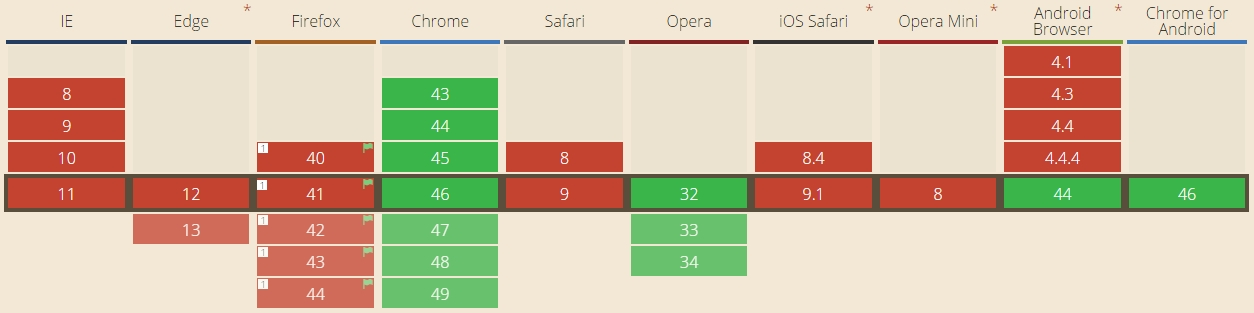
\includegraphics[width=\linewidth]{kapitel2/bilder/5-html-imports-browserunterstuetzung}
 \caption{Browserunterstützung der HTML Imports}
 \label{fig:bdhtmli}
\end{figure}
